\documentclass[a4paper,10pt]{article}
\usepackage[utf8]{inputenc}
\usepackage{graphicx}
\usepackage{subfigure}
\usepackage{caption}
\usepackage{amsmath}
\usepackage[bookmarks=true]{hyperref}
\usepackage{amssymb}


\title{\textbf{Nonlinear Model Order Reduction using POD/DEIM for Optimal Control of Burgers' Equation}}
\author{\href{mailto:manuelmbaumann@gmail.com}{Manuel M. Baumann}}
\date{July 15, 2013}

\begin{document}
\maketitle

\noindent
In my Master thesis I consider the following optimal control problem,
\begin{equation}
\label{objFun}
\min_u \frac{1}{2} \int_0^T \int_0^L [y(t,x) - z(t,x)]^2 + \omega u^2(t,x) \ dx \ dt, \quad \omega \in \mathbb{R}_+,
\end{equation}
where $y$ is the solution of the nonlinear, unsteady Burgers' equation with homogeneous Dirichlet boundary conditions and given initial condition $y_0(x)$,
\begin{equation}
\label{Burgers2}
\begin{split}
y_t + \left( \frac{1}{2}y^2 - \nu y_x\right)_x = f + u&, \quad (x,t) \in (0,L) \times (0,T), \\
y(t,0) = y(t,L) = 0&, \quad t \in (0,T), \\
y(0,x) = y_0(x)&, \quad x \in (0,L),
\end{split}
\end{equation}
and $u$ being a control such that \eqref{objFun} is small and, hence, the solution of Burgers' equation is close to the desired state $z$. This problem has been considered in \cite{H08} and the authors of \cite{KV99} proposed the well-known method of Proper Orthogonal Decomposition (POD) in order to reduce the computational cost of the optimization algorithm which solves \eqref{objFun}-\eqref{Burgers2}.

In my thesis work, the Discrete Empirical Interpolation Method (DEIM), introduced by \cite{DEIM} in $2010$, has been used for the first time in the context of optimal control for Burgers' equation in order to further improve the computational benefit of POD and solving \eqref{objFun}-\eqref{Burgers2} on a POD-DEIM reduced model.
\begin{figure}[h!]
\centering
%\subfigure{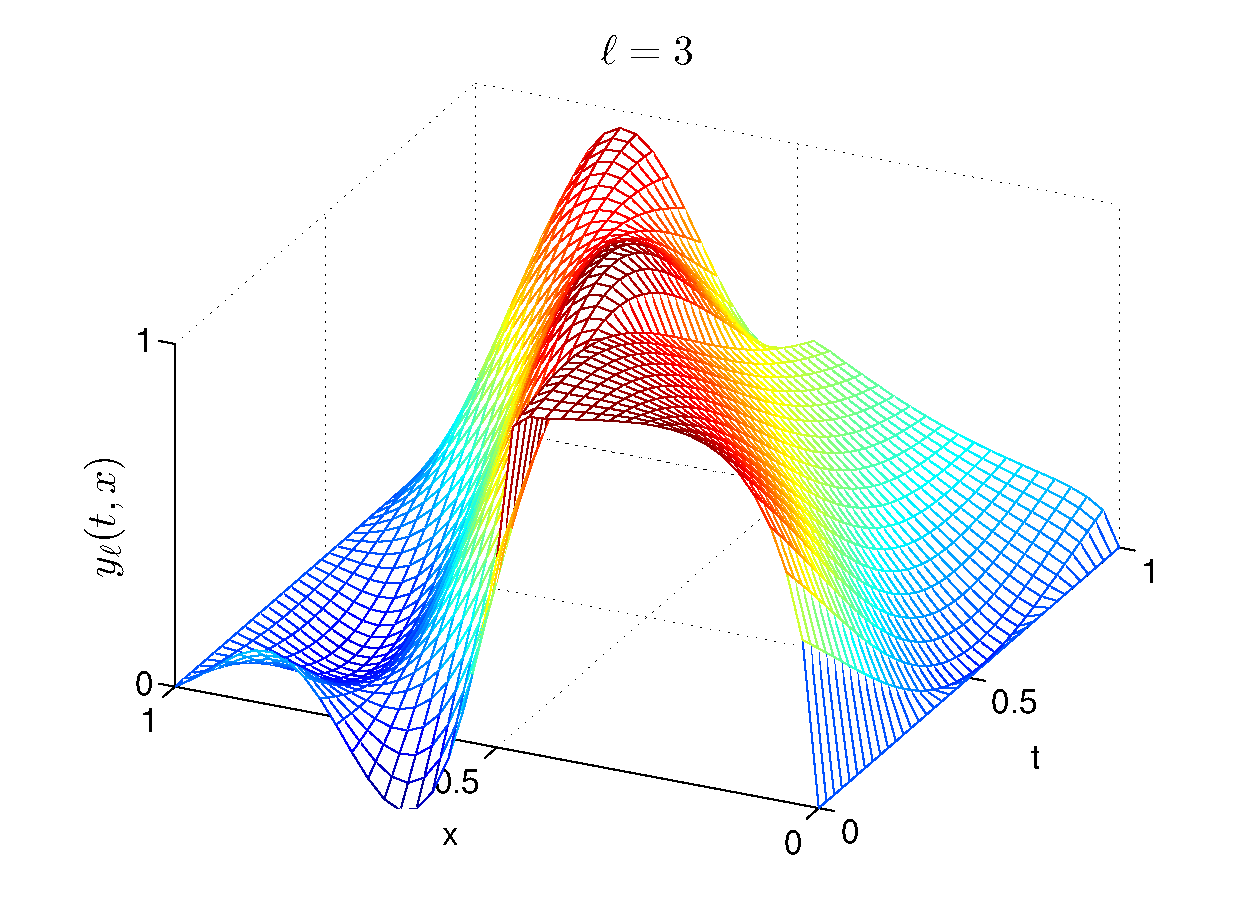
\includegraphics[width=0.4\textwidth]{plots/l3}}
\subfigure{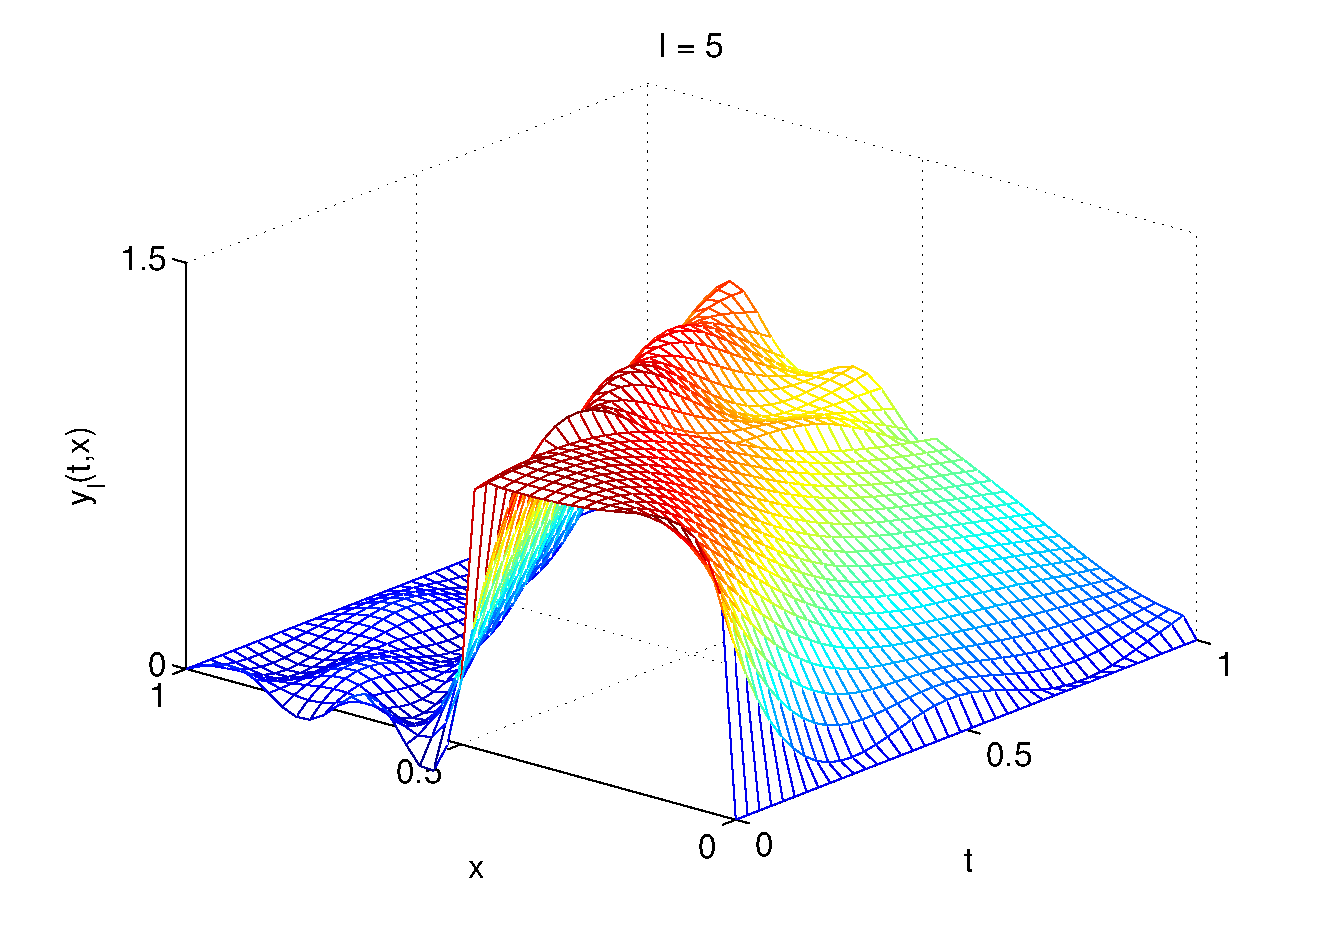
\includegraphics[width=0.4\textwidth]{plots/l5}}
%\subfigure{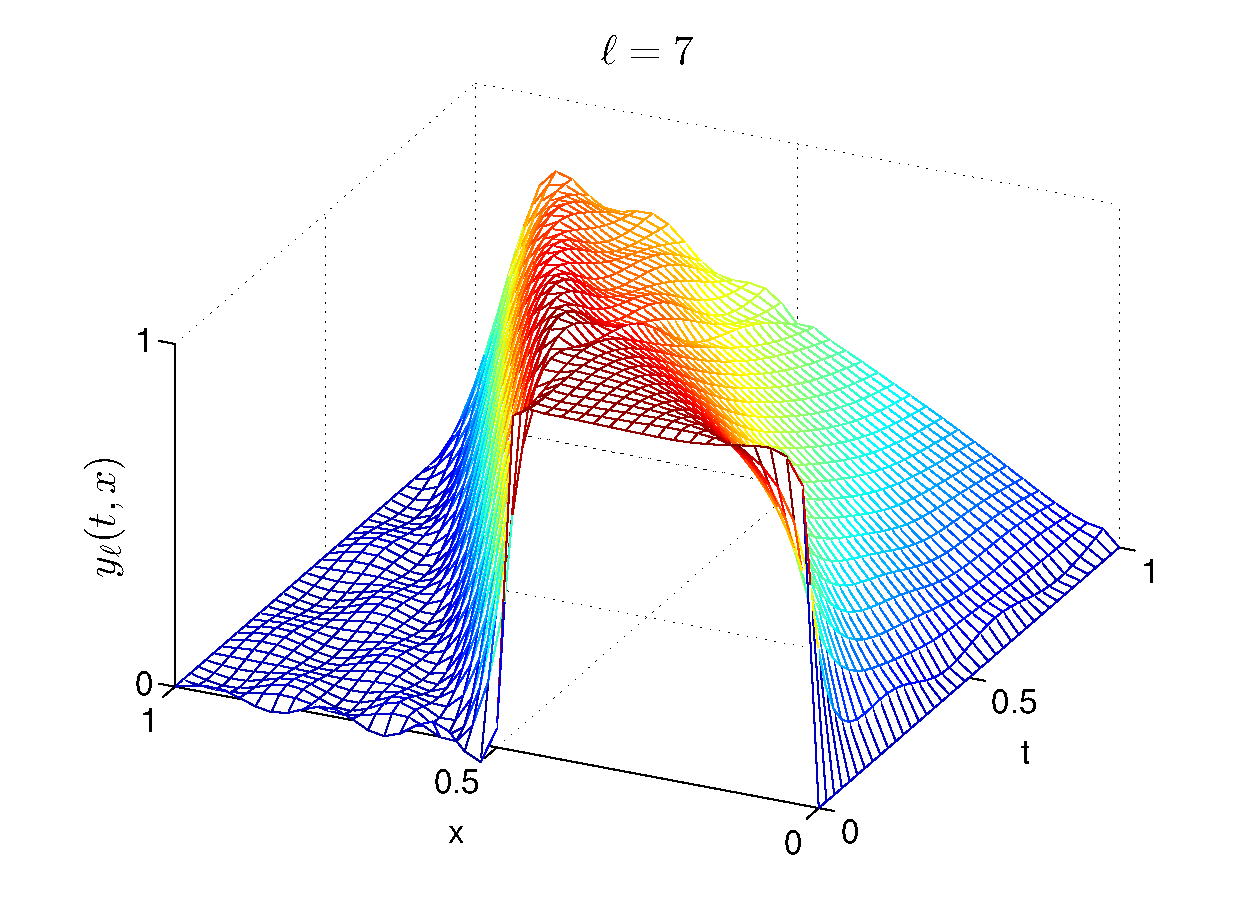
\includegraphics[width=0.4\textwidth]{plots/l7}}
\subfigure{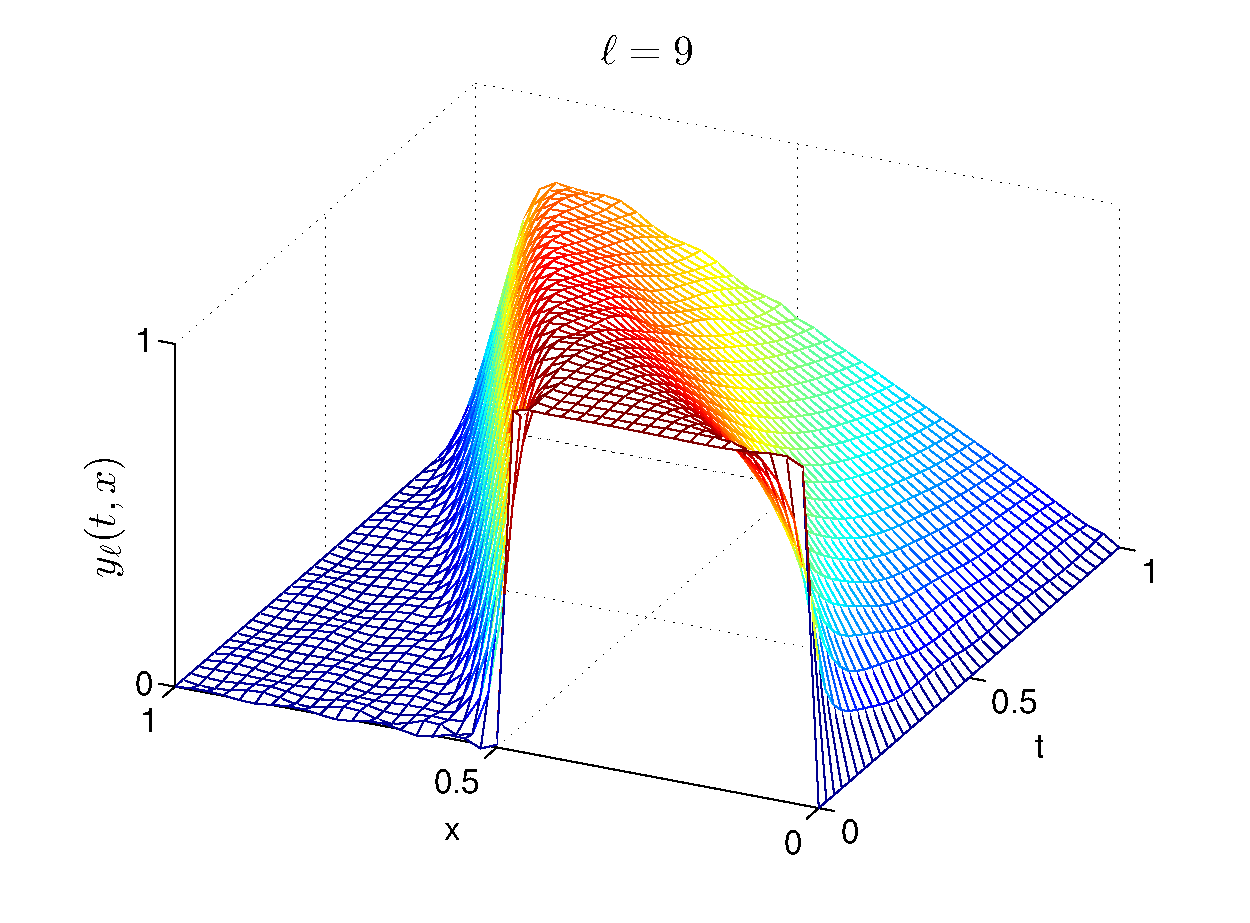
\includegraphics[width=0.4\textwidth]{plots/l9}}
\caption{POD-DEIM approximations of the uncontrolled ($u \equiv 0$) Burgers' equation for two different reduced dimensions $\ell$.}\label{PODplot}
\end{figure}

\newpage
\bibliographystyle{plain}
\bibliography{LitStudy}
\end{document}
